\documentclass{article}

\setlength{\paperwidth}{210mm}
\setlength{\paperheight}{297mm}
\setlength{\hoffset}{-12mm}
\setlength{\voffset}{-10mm}
\setlength{\evensidemargin}{0mm}
\setlength{\oddsidemargin}{0mm}
\setlength{\topmargin}{0mm}
\setlength{\headheight}{0mm}
\setlength{\headsep}{5mm}
\setlength{\textheight}{256.2mm}
\setlength{\textwidth}{184.2mm}
\setlength{\marginparsep}{0mm}
\setlength{\marginparwidth}{0mm}
\setlength{\footskip}{5mm}
\setlength{\marginparpush}{0mm}


\usepackage[spanish]{babel}
\usepackage[utf8]{inputenc}
\usepackage{graphicx}

\pagestyle{myheadings}
\markright{IA - Práctica de búsqueda local}

\title{\Huge{Práctica de búsqueda local} \\
\vspace{15mm}
   \Large{Laboratorio de Inteligencia Artificial}}
\author{Marion Not - Michael Boris Mandirola}
\date{Primavera 2010-2011}

\begin{document}
\maketitle
\newpage
\tableofcontents
\newpage
\section*{Introducción}
El objetivo de esta práctica es analizar y resolver un problema de optimización
logistica mediante algoritmos de búsqueda local. Definiremos la representación
del problema como estado y estudiaremos la influencia de los elementos que
intervienen en esta búsqueda y que hemos visto a clase (estado inicial, función
heurística y operadores) bajo diferentas condiciones sobre los parametros del
problema.

Usaremos dos tipos de algoritmos de búsqueda local : el Hill Climbing y el
Simulated Annealing. Como el objectivo de la práctica no es la implementación de
estos algoritmos, usaremos las herramientas proporcionadas por el package AIMA. 
En el caso del Simulated Annealing, tambien estudiaremos la influencia de los 
parametros del algoritmo.

\section{Representación del problema}
El contexto del problema es el siguiente : Una empresa de transporte esta
contratada por una compania para gestionar el encaminamiento de productos desde
un almacen central hasta unos centros de producción.

Cada dia, los centros realizan un conjunto de peticiones de diferentes tipos y 
cantidades de productos que se tienen que entregar a una cierta hora. El pago se
realiza en función de la cantidad de productos entregados y la puntualidad con
la cual han llegado al centro.

La empresa de transporte quiere optimizar estas entregas. Solucionaremos este
problema para un dia dado.

\subsection{Identificación de los elementos relevantes}
%descripcion, analisis y caracteristicas del problema
Para cada problema, tendremos unos elementos constantes, unos elementos
especificos del problema y unos elementos variables que se tendran que
determinar para llegar a la solución.

\subsubsection{Constantes}
\begin{description}
\item[Centros de producción :] Como lo hemos dicho, el numero de centros esta 
fixado a 6.
\item[Horas de entrega :] Las entregas se haran a cada hora en punto del dia. La
primera se hara a las 8 y la ultima a las 17, para un total de 10 horas de
entrega.\\
El retraso en la entrega de una peticion es simplemente la diferencia entre la
hora de entrega deseada y la efectiva. Si la peticion no esta entregada en el
dia, el retraso es la diferencia entre la hora de entrega deseada y las 8 del
dia siguiente. No obstante, como solucionemos el problema solo para un dia, no
se tendra que gestionar la entrega de estas peticiones el dia siguiente.
\item[Transportes :] Tendremos un transporte para cada hora del dia y cada
centro, es decir 60 transportes en total. La capacidad de los camiones usados
sera de 500, 1000 o 2000kgs, en proporción variable.\\
No tenemos que gestionar la recogida de productos en el almacen, ni el recorrido
de los transportes, ni la cantidad de camiones fisicos que se necesitan :
Suponemos que la empresa dispone de una flota suficiente para hacer todas las
entregas en tiempo.
\item[Peticiones :] Las peticiones se haran para una de las horas de entregas y
para una cantidad de productos de 100, 200, 300, 400 o 500kgs.\\
El precio pagado para cada peticion entregada sera el indicado en la tabla 1
menos unos 20\% del mismo para cada hora de retraso, es decir que para mas de 5h
de retraso le tocara pagar a la empresa de transporte. Si una peticion no esta
entregada en el dia, la empresa de transporte tendra que pagar el precio de la
peticion mas unos 20\% para cada hora hasta las 17.
\begin{center}
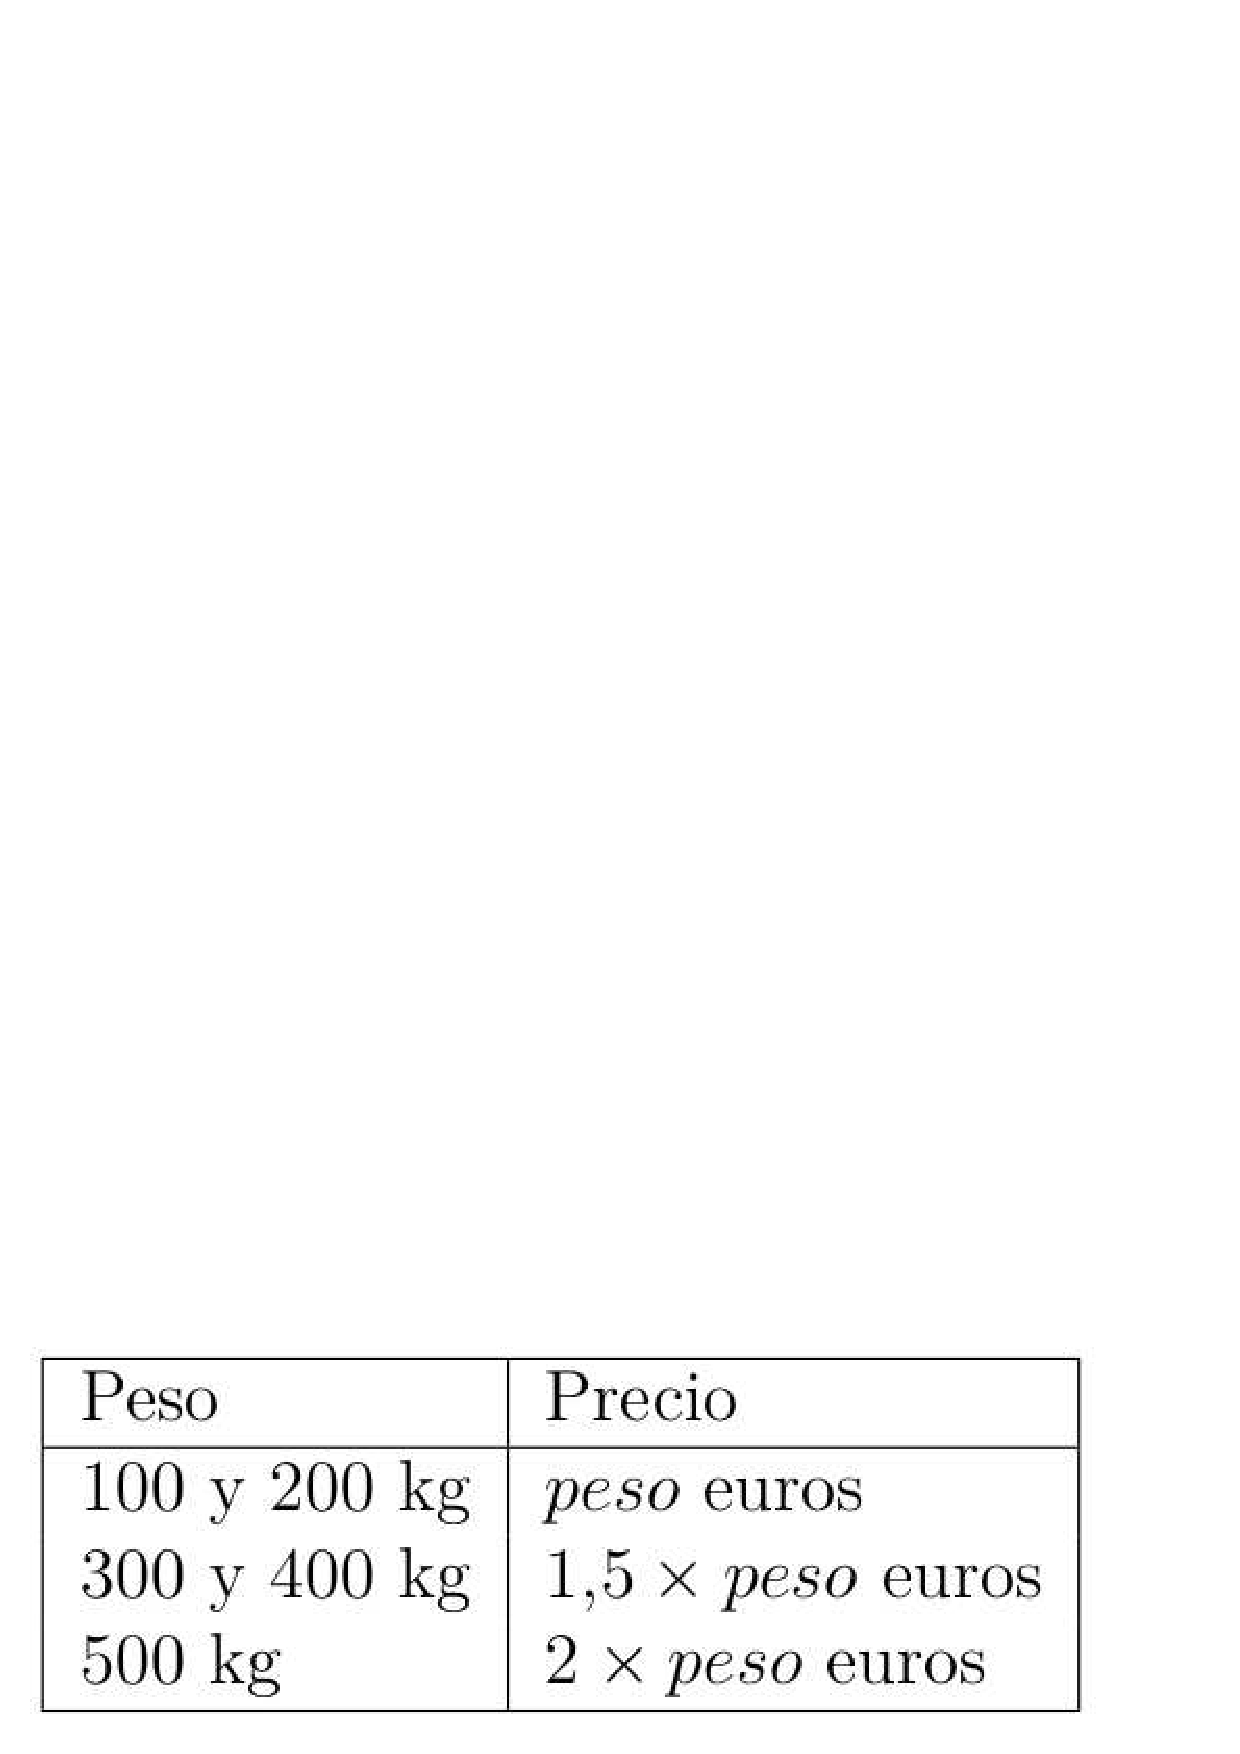
\includegraphics[width=3cm]{preciosEntregas}\\
{\it Tabla 1 : Precio de las entregas.} \end{center}
\end{description}

\subsubsection{Elementos de la solucion}

\subsection{Estado}
\subsubsection{Elementos del estado}
%descripcion detallada y justificacion
\subsubsection{Tamaño del espacio de búsqueda}


\subsection{Operadores}
%descripcion detallada, condiciones de aplicacion, efecto
%factor de ramificacion
%justificacion de la eleccion
\subsubsection{Desplazamiento de una petición dentro de un centro}
\subsubsection{Intercanvio de capacidades de camiones}
\subsubsection{Operadores no implementados}


\subsection{Funciones Heurísticas}
%descripcion y analisis de los factores que intervienen en las heuristicas
%justificacion de la eleccion de estas heuristicas y de las ponderaciones
%explicacion del impacto de las heuristicas en la busqueda
\subsubsection{Maximización de la ganancia}
\subsubsection{Minimización de la diferencia entre hora de entrega deseada y
efectiva}


\subsection{Estados Iniciales}
%justificacion de la eleccion de los estados (bondad de la solucion, coste,
% adaptacion a cada algoritmo)
%descripcion de la implementacion

En un primer momento hemos intentado generar estados diferentes con lógicas muy diferentes con la idea de buscar nuestros estados iniciales entre un grupo más amplio y en particular elegir dos estados que tengan características muy diferentes. Es decir tiempo de generación de el estado inicial, complejidad de el algoritmo, posibilidades de evolución, calidad de la solución buscada.

\subsubsection{a}
A) Este estado divide los camiones de manera ecua entre los centres asignando los camiones con mas capacidad a los transportes mas tempranos. Las entregas están entregadas lo mas pronto posible: se hace una lista de peticiones pertinentes a un centro, se ordenan crecientemente por tiempo de entrega y disminuyendo por precio y se pasa toda la lista poniendo las peticiones en el transporte más pronto que tiene más tiempo libre.

\subsubsection{b}
B) Este estado ordena las peticiones por precio y hora. Por cada petición, intenta entregarla en la hora pertinente con este algoritmo:
Si no hay camión, se pone el camión disponible más pequeño y la petición, si hay camión y bastante capacidad libre también se pone la petición. Si hay camión de capacidad inferior a la capacidad máxima y hay disponibilidad de camiones más grandes, se asigna un camión mas grande en lugar de lo más pequeño y se pone la petición. Además, si no hay camiones libres más grandes intenta hacer lo mismo en las horas más tempranas hasta las 8. Si no tiene éxito, intenta hacerlo en las horas después hasta las 17.
Después si hay oras sin camión, se asignan los camiones que se quedan libres.

\subsubsection{f}
F) Los camiones se asignan como en el estado A. Sin ordinación se iteran todas las peticiones intentando ponerlas en su hora de pertinencia. Después, iterativamente por cada petición se intenta poner, las que se quedan no entregadas, en las horas más tempranas de la suya hasta las 8 y si no se tiene éxito, se intenta hacerlo en las horas después hasta las 17.

\subsubsection{v}
V) Los camiones se asignan como en el estado A. Las peticiones se quedan todas no entregadas.


\section{Implementación}

\subsection{Generación de problemas aleatorios}

\subsection{Uso del AIMA}

\subsection{Ejecucción de tests}
%input y script

\subsection{Recuperación de resultados}
%output


\section{Resultados}
% explicaciones y analisis detallada
% comparar los resultados con lo que se esperaba
% hacer los experimentos del enunciado y contestar las preguntas
% hacer tb mas experimentos para complementar

\subsection{Influencia de la solución inicial}
%coste de creacion
% influenca en la bondad de la solucion y en el coste del algoritmo

\subsection{Influencia de los operadores}
% comparacion entre conjuntos de operadores
% impacto sobre el coste temporal y bondad de la solucion

\subsection{Influencia de la heurística}
% comparacion entre las dos heuristicas, impacto en tiempo y bondad de solucion
% hacer experimentos para ver la influenca de las ponderaciones

\end{document}
